% An example second appendix from the example thesis thesis.tex.
\chapter{EE 518 Test Results}

\section*{E E 518 Lab Tests}

Further testing of the square-law detector was performed by using the radiometer in a real world event.  This test was exercised in conjunction with the Microwave Remote Sensing class (E E 518) under Dr. Brian Hornbuckle.  In the Spring of 2012 the radiometer was moved to the roof of agronomy and the EE 518 students conducted a number of tests using the N200 software defined radio to collect the data.


{\begin{figure}[h!tb] 
\centering
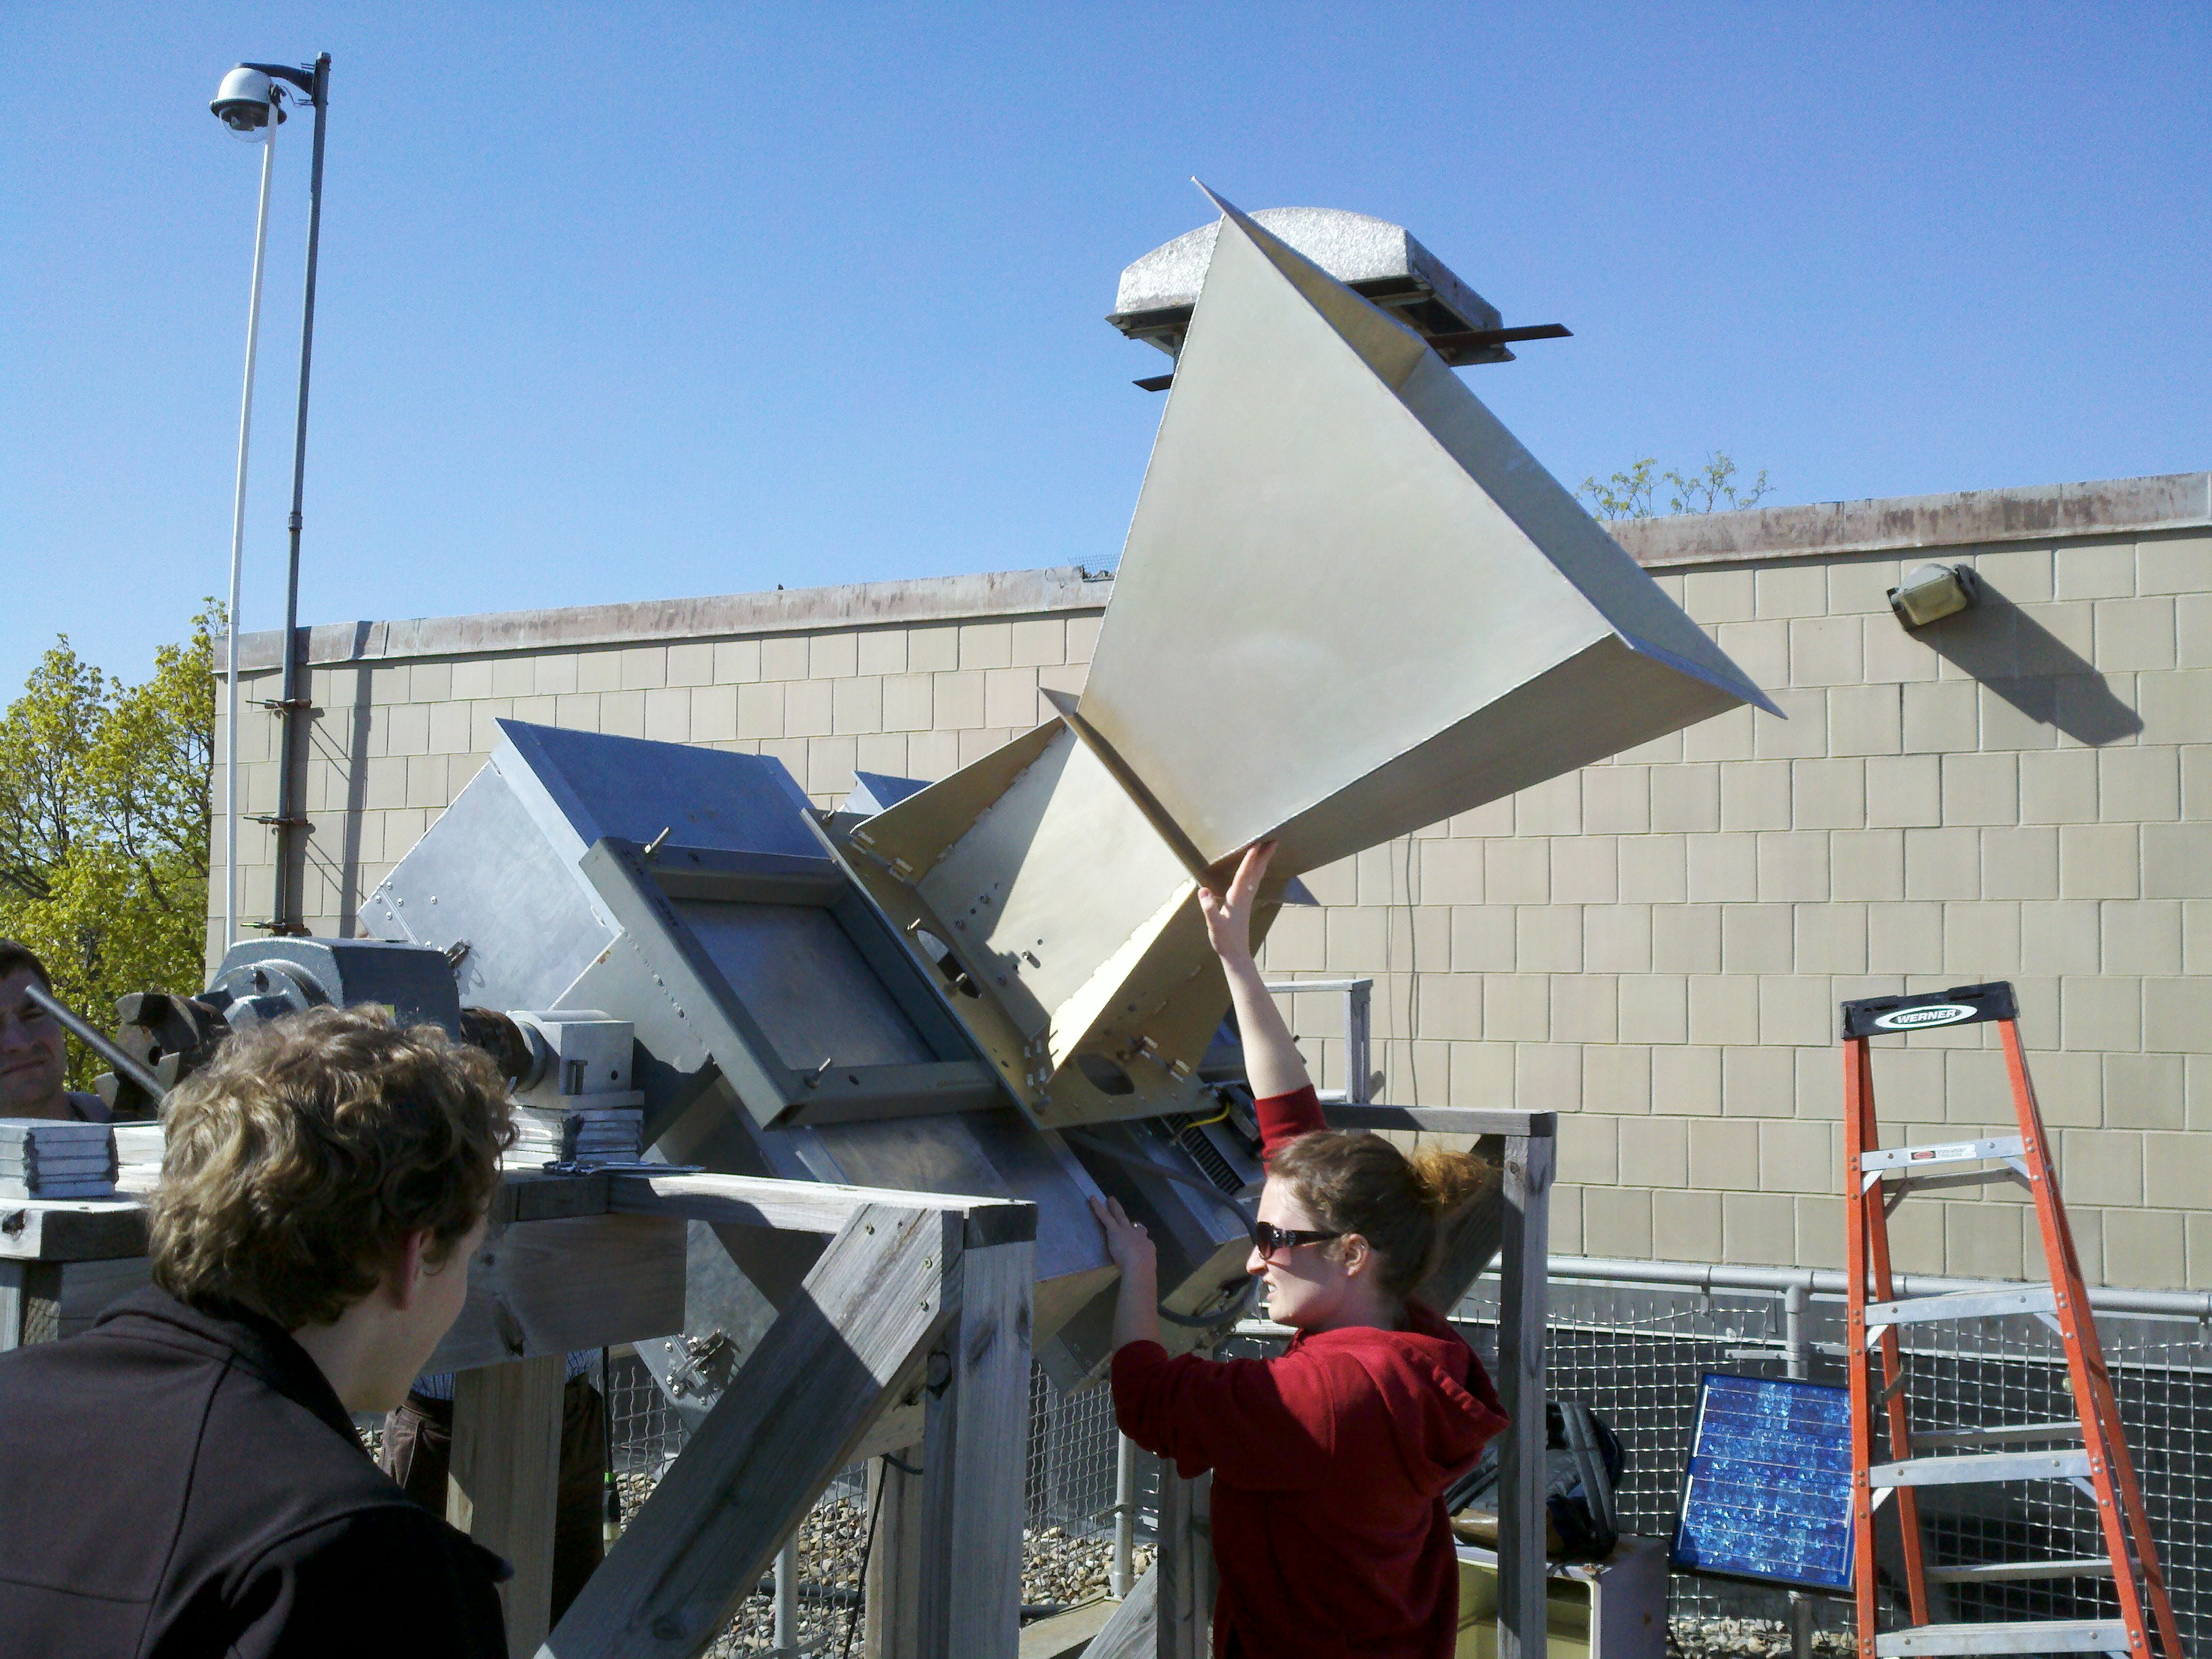
\includegraphics[width=\textwidth]{Images/radiometer_roof.jpg}
\isucaption{Students rotating the radiometer for an experiment on Agronomy Hall}
\label{radiometer_roof}
\end{figure}
}

The E E 518 test however showed that there were additional problems with the radiometer.  While the test showed that the SDR could in fact read data, the data was skewed.  It was later found out that the radiometer was generating an interfering signal that caused the power readings to be elevated.  It was also found that the interfering signal was also flucatating and seemed to correspond somewhat to the physical position of the radiometer.  This was found as a result of having the SDR record the raw I/Q values and then was analyzed later.  Through this analysis, we found that a strong harmonic was developed and caused a spike in signal being recorded.  Although the exact reason for this has not been found, the problem has been isolated to something in the RF Front End of the ISU radiometer. 

In the Spring of 2014 the E E 518 class ran another experiment, but this time a different one.  This experiment mimicked the experiments that the author ran to calibrate and test the radiometer.  This allowed an outside source to validate the results that I was getting with running the radiometer.  Like my tests, the students submerged a matched load into liquid nitrogen and then in boiling water.  The liquid nitrogen was assumed to be at 77 K and the boiling water was measured to be at 99 C or 372 K.  The students were then given a mystery sample in which they had to determine the temperature of a water sample.  Since the students had to points, they could find the calibration line and determine the temperature.  The experiment was run twice as we expected the radiometer may have drifted between measurements.  

\subsection{Test setup}
For the E E 518 class, the setup was similar to experiments that was run to test the results in this thesis.  For the E E 518 however the students only used the N200 SDR for recording the total power readings.  The ISU Radiometer was used only to provide the RF front end as in other tests and the output from that RF front end was feed into the N200.  A matched load was attached to the input of the RF front end.  This matched load was then submersed into either the liquid nitrogen or water baths.  

\subsection{Lab Experiment}

Students conducted the experiment by submerging the matched load into Liquid Nitrogen, then boiling water, then an unknown sample.  The LN2 was believed to be at 77 K.  The boiling water was measured by the students and was recorded to be 99 C.  The mystery water was then measured by myself and recorded both before the students placed the match load in there and after to see if it changed temperature between the experiments.  During this time the GNURadio program that I wrote recorded the total power information to the hard drive.  This file was then given to the tests and an example Matlab script was also provided for them to use to read the data file.

\subsection{Lab Results}

Two labs were conducted, however the data from the first lab was more stable and had better results than the second lab.  Therefore the students only used the data set from the first lab experiment.  Students were then asked to write a lab report that calculated the temperature of the mystery water, write up what each component in the radiometer does, plot the raw rQ values, calculate and plot the calibration lines and finally calculate the NE$\delta$T for the system by doing a standard deviation on a section of the data that was at a stable temperature.  

The results of the lab experiments were mixed in the students reports.  Almost all of the students reported a temperature cooler than the actual recorded temperature.  After looking at the data and the student reports, there is a couple of reasons this may have happened.  First, it would appear that there may not have been enough time to allow the matched load to equalize.  The graph of the rQ values does not show a stable line as expected with the LN2 and hot water baths.  It appears that there was a dip in the rQ values and that the students picked that lowest point as the mystery water temperature.  It is uncertain what caused the dip.  Second, it is safe to say that the temperature of the mystery water changed due to the matched load being inserted in it.  There was nothing to keep the mystery water at a fixed temperature as it was simply water at room temperature.  These may have caused some of the odd readings and made it difficult for the sample to stabilize unless it was allowed to sit longer.

\subsection{Conclusion}
While the students were not able to get an accurate reading of the mystery water, the calibration points, and NE$\delta$T values were within what was expected of the system and matched fairly close to those calculated by the author.  Overall, this experiment proved to be a good exercise for the students as it allowed them to have a hands on exercise and see and operate a radiometer for themselves.   